\documentclass[]{article}

\usepackage{graphicx}

%opening
\title{%
	Project 2 Analysis\\
	\large Run Times of Sorting Algorithms}
\author{Phillip Janowski}

\begin{document}

\maketitle

\section{Theoretical Time Complexities}
\begin{center}
	\begin{tabular} {|l|c|c|c|}
		\hline
		Algorithm & Best Case & Average Case & Worst Case\\
		\hline 
		Quick Sort & $ O(n \log(n)) $ & $ O(n\log(n)) $ & $ O(n^2) $\\
		\hline
		Merge Sort & $ O(n \log(n)) $ & $ O(n\log(n)) $ & $ O(n \log(n)) $\\
		\hline
		Bubble Sort & $ O(n) $ & $ O(n^2) $ & $ O(n^2) $\\
		\hline
		Bubble Sort With Swap Counting & $ O(1) $ & $ O(n \log(n)) $ & $ O(n^2) $\\
		\hline
		Insertion Sort & $ O(n) $ & $ O(n^2) $ & $ O(n^2) $\\
		\hline
		Selection Sort & $ O(n^2) $ & $ O(n^2) $ & $ O(n^2) $\\
		\hline
	\end{tabular}
\end{center}

\section{Observed Times}
\centerline{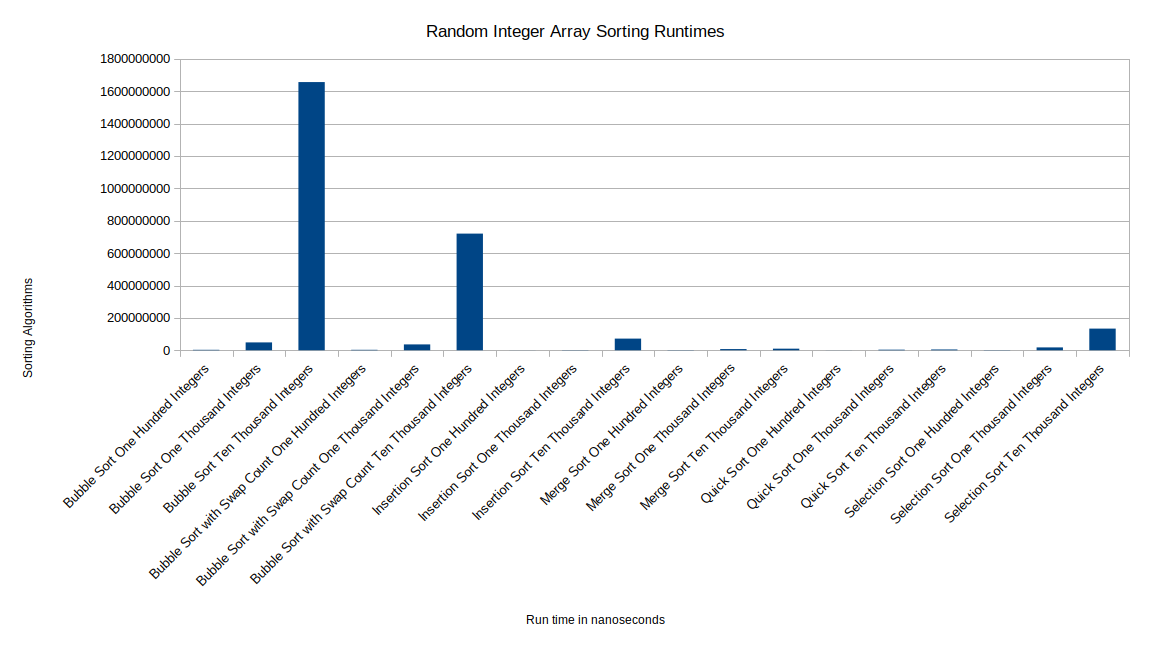
\includegraphics[scale=.7]{randomIntegerTimes}}
\centerline{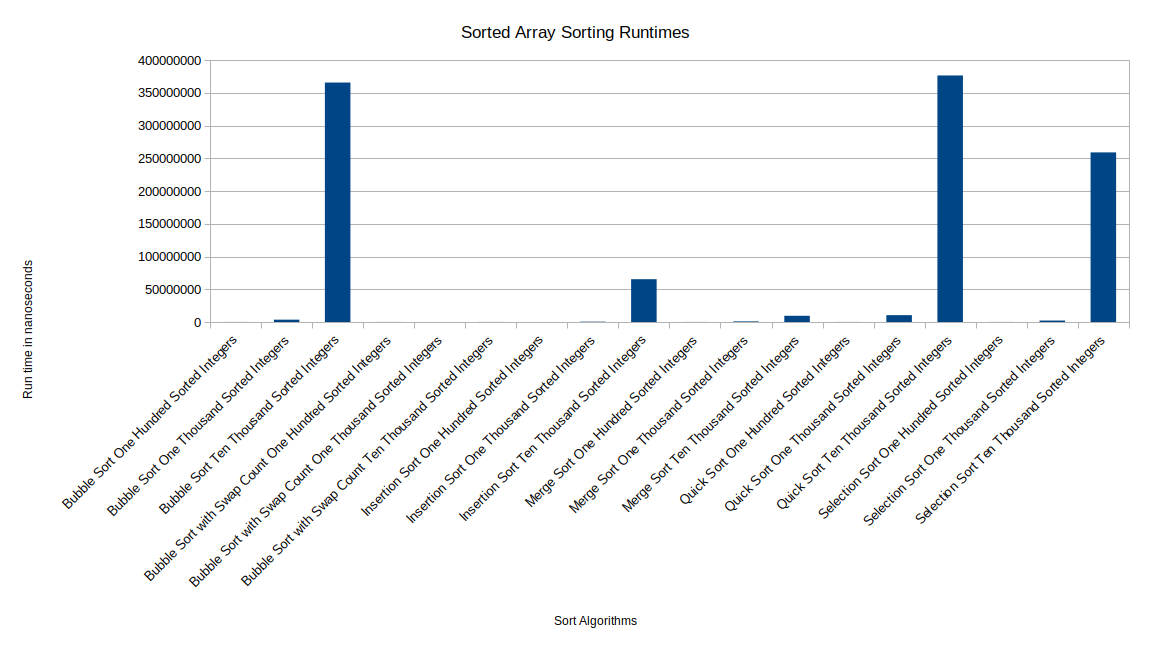
\includegraphics[scale=.7]{sorted}}
\centerline{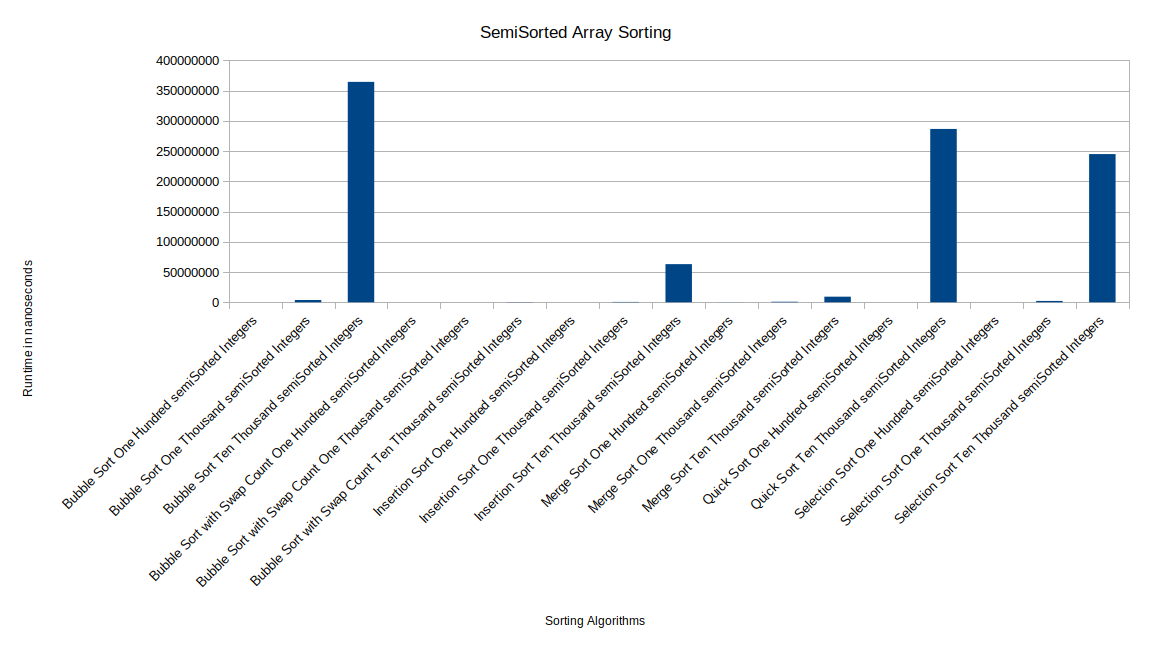
\includegraphics[scale=.7]{semisorted}}
\centerline{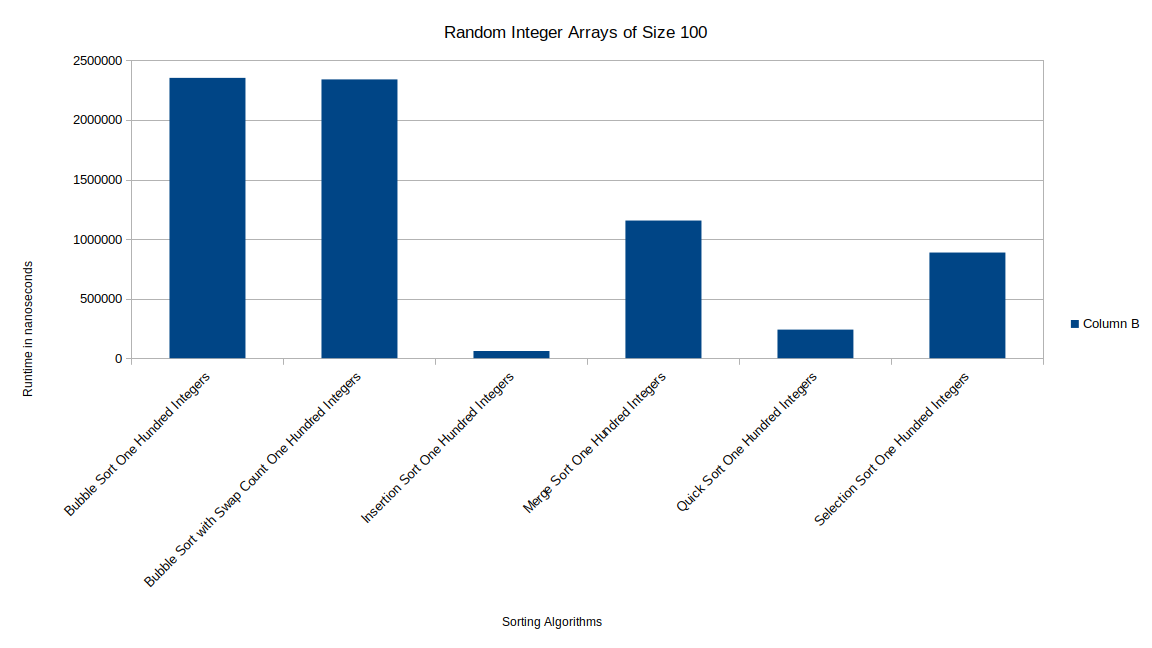
\includegraphics[scale=.5]{random100}}
\centerline{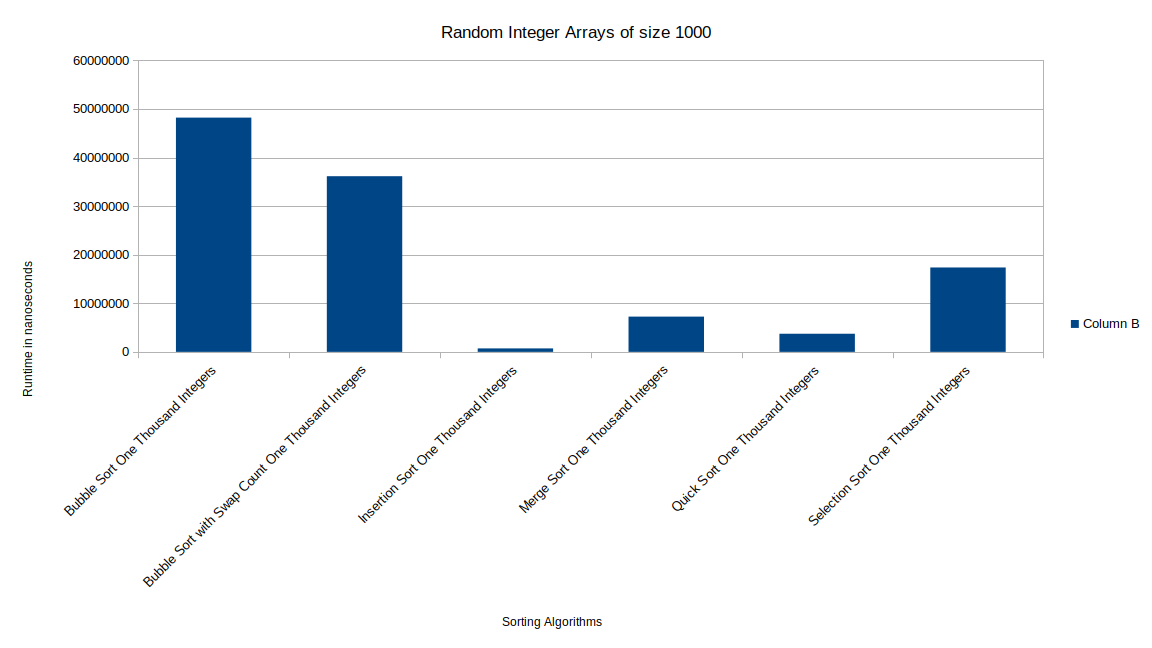
\includegraphics[scale=.5]{random1000}}
\centerline{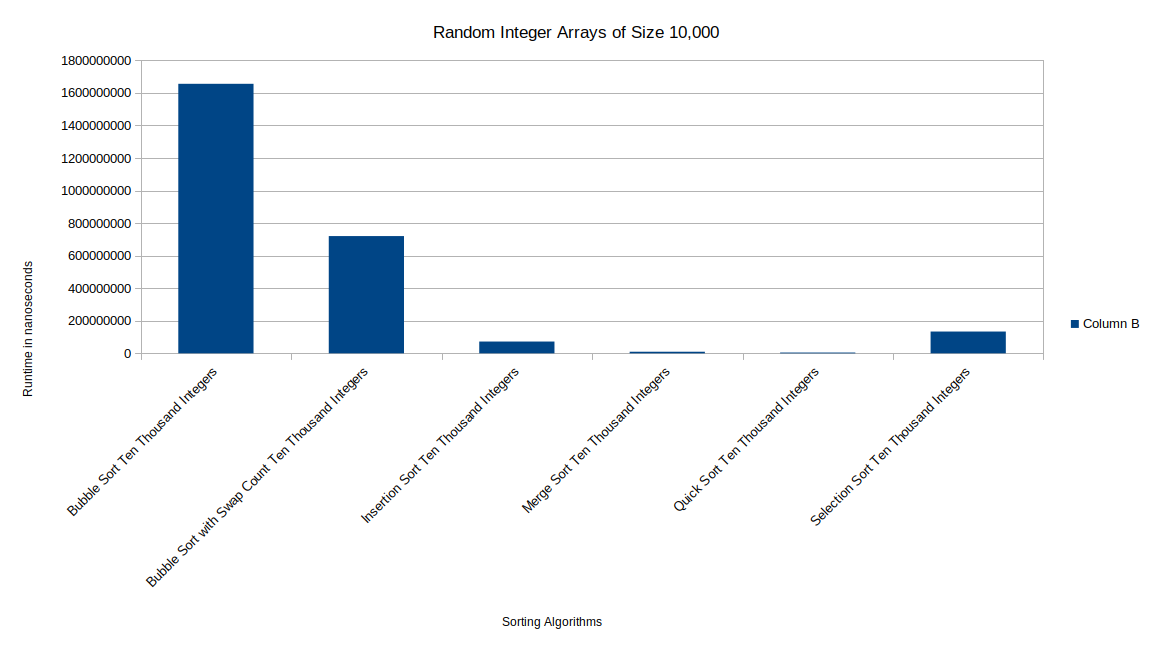
\includegraphics[scale=.5]{random10000}}
\centerline{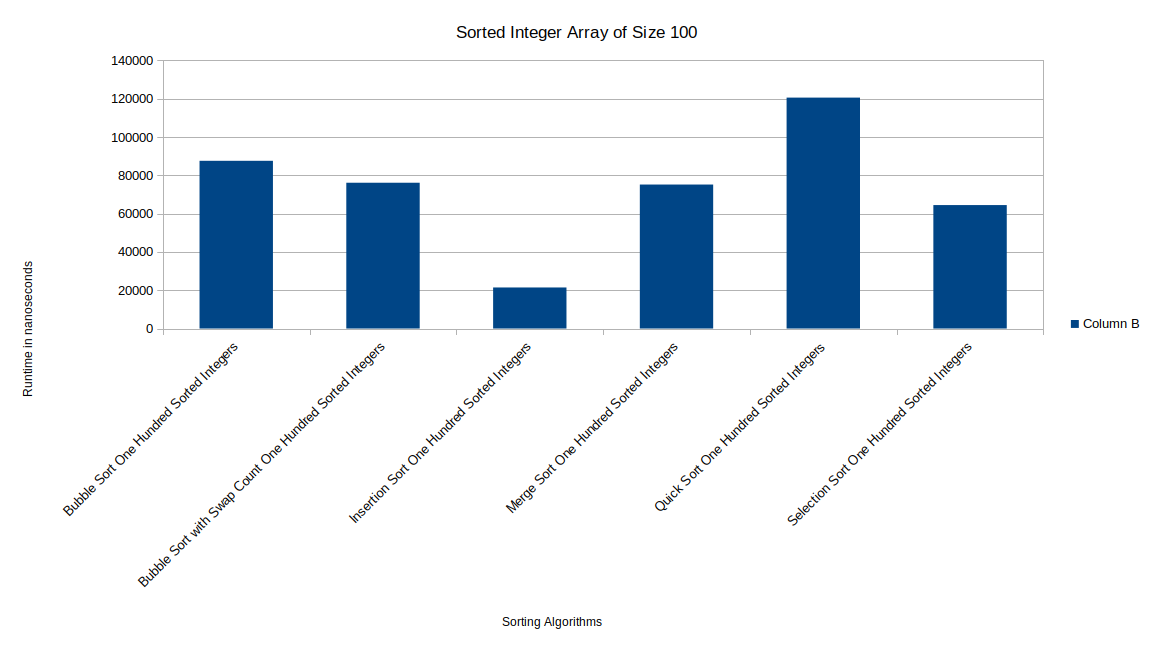
\includegraphics[scale=.5]{Sorted100}}	
\centerline{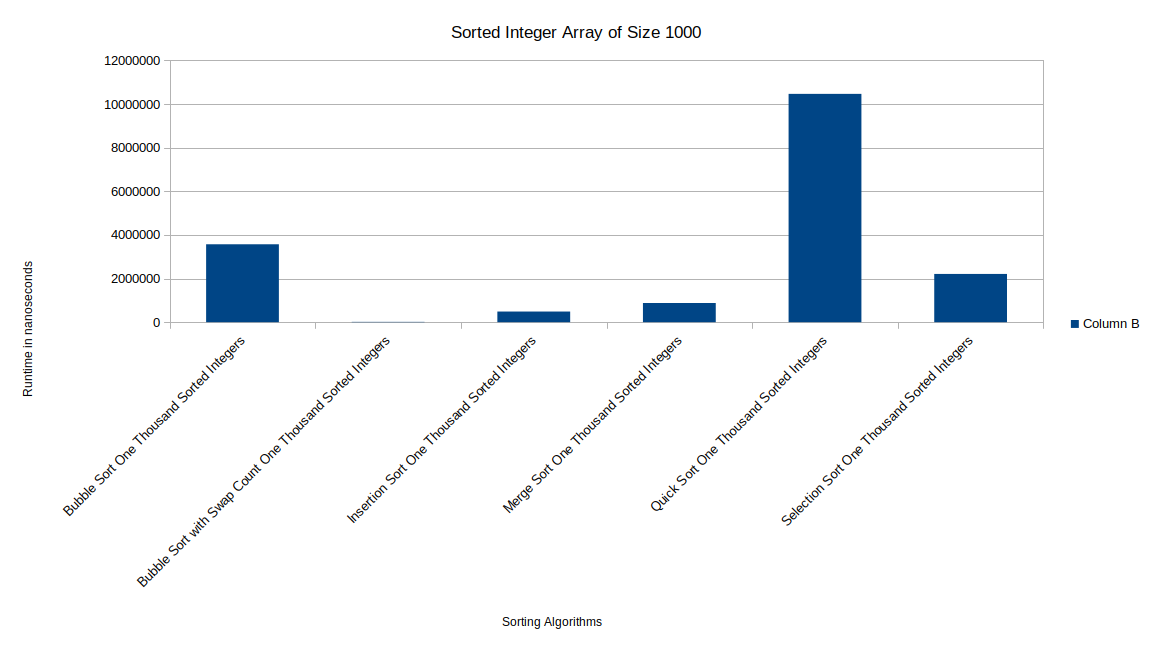
\includegraphics[scale=.5]{Sorted1000}}
\centerline{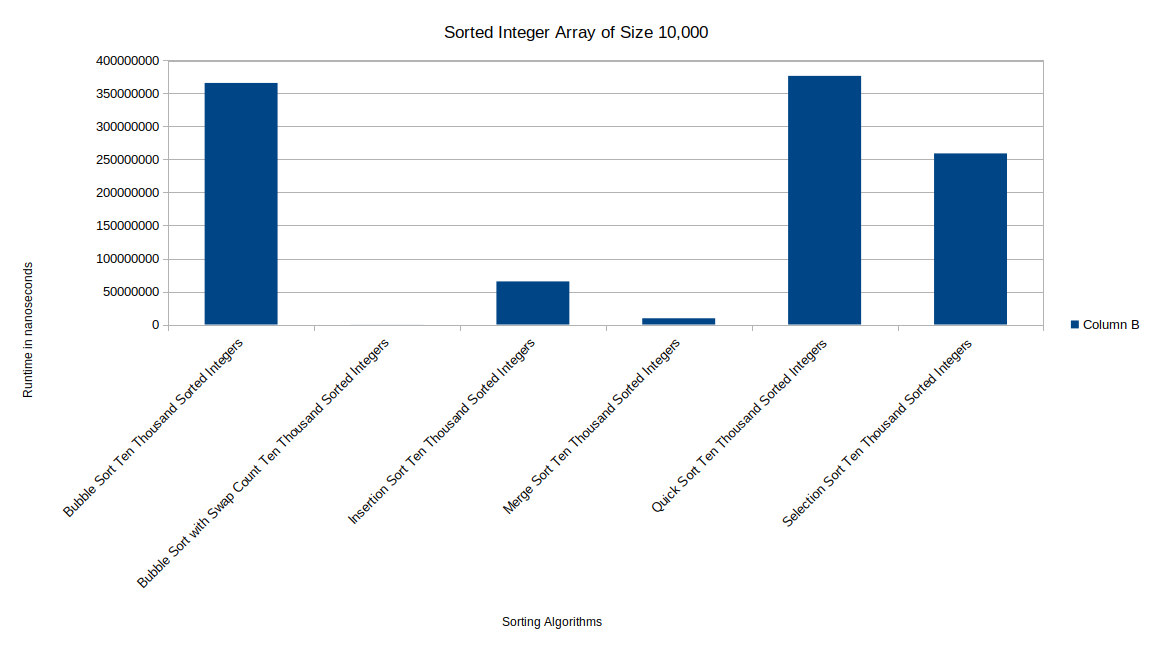
\includegraphics[scale=.5]{Sorted10000}}
\centerline{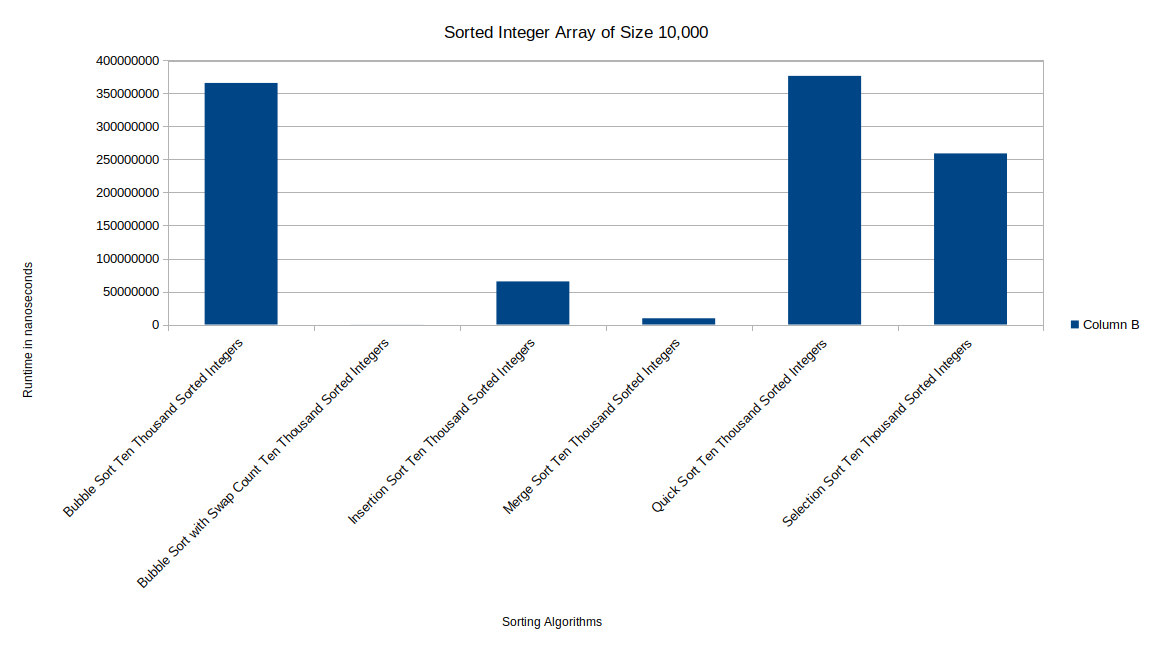
\includegraphics[scale=.5]{Sorted10000}}
\centerline{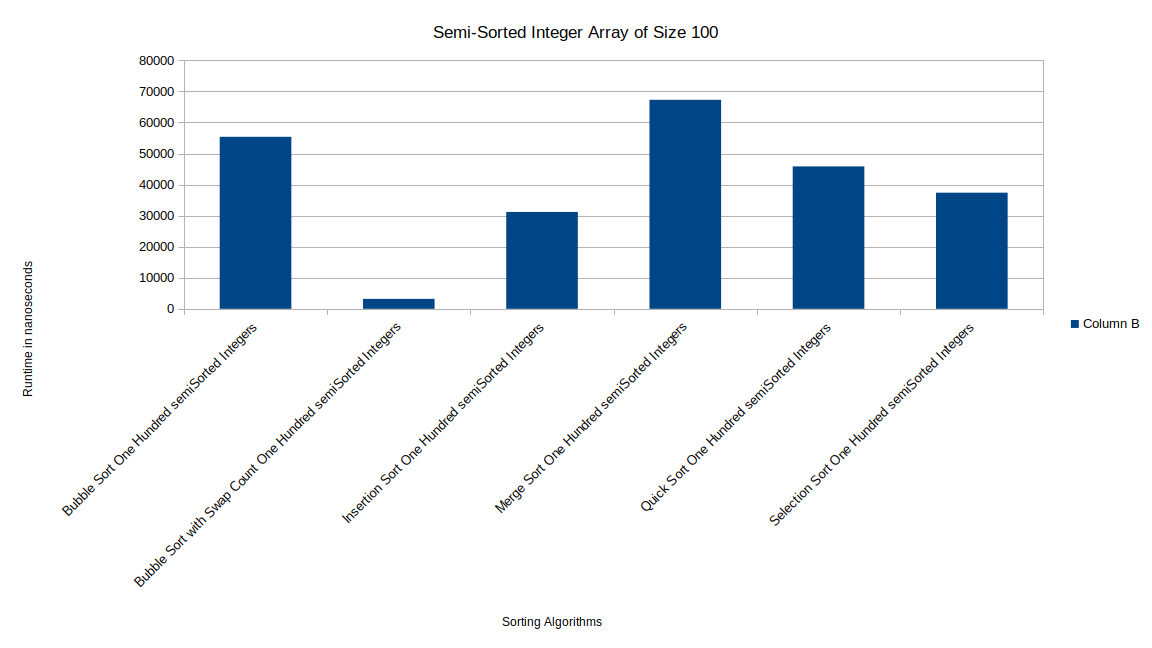
\includegraphics[scale=.5]{semiSorted100}}
\centerline{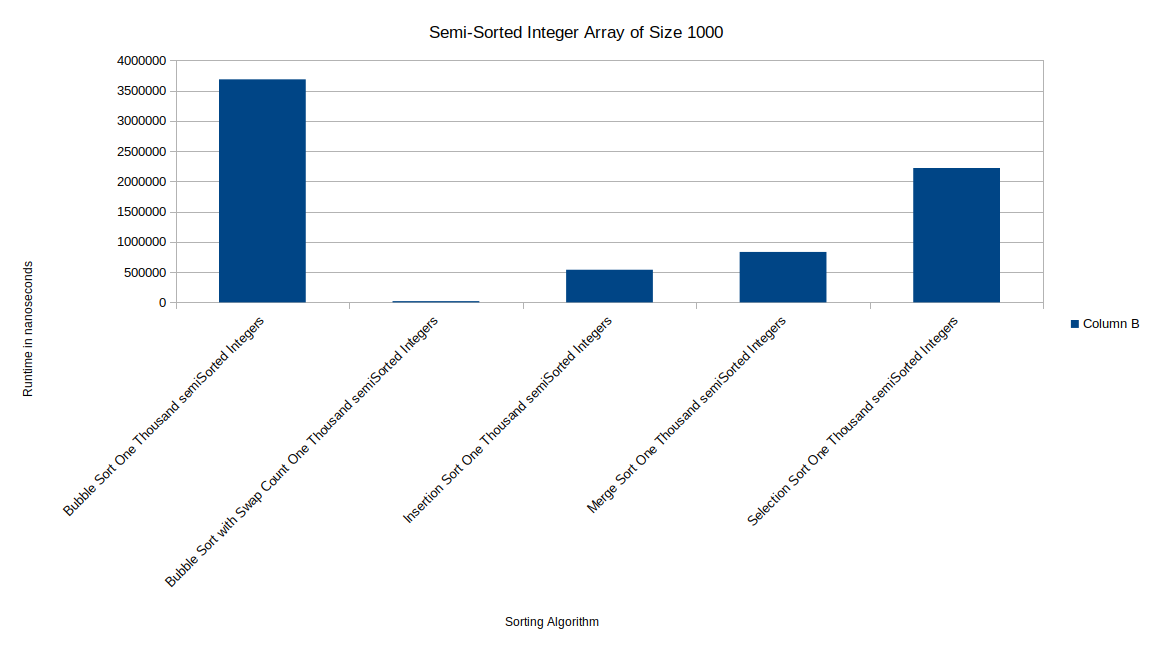
\includegraphics[scale=.5]{semiSorted1000}}
\centerline{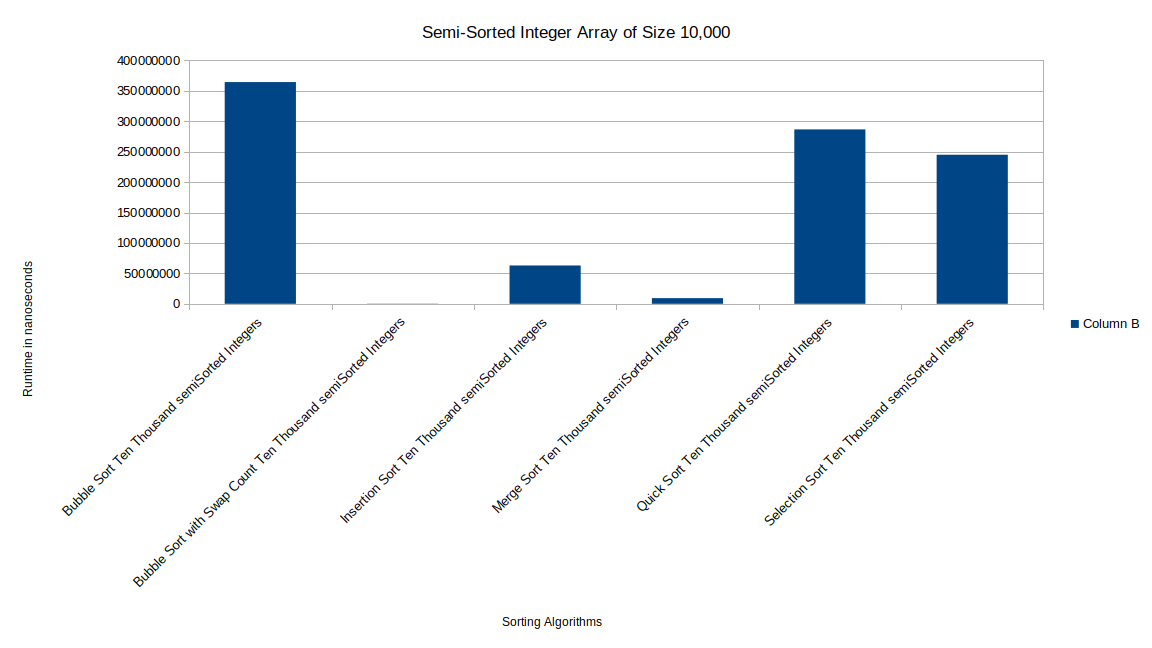
\includegraphics[scale=.5]{semiSorted10000}}


\section{Raw Data}

	\begin{tabular}{|l|c|}
		\hline
		Bubble Sort One Hundred Integers & 2340277\\
		\hline
		Bubble Sort One Hundred Sorted Integers & 87578\\
		\hline
		Bubble Sort One Hundred semiSorted Integers & 55402\\
		\hline
		Bubble Sort One Thousand Integers & 36158542\\
		\hline
		Bubble Sort One Thousand Sorted Integers & 3570585\\
		\hline
		Bubble Sort One Thousand semiSorted Integers & 3687019\\
		\hline
		Bubble Sort Ten Thousand Integers & 1655832010\\
		\hline
		Bubble Sort Ten Thousand Sorted Integers & 365890163\\
		\hline
		Bubble Sort Ten Thousand semiSorted Integers & 364328717\\
		\hline
		Bubble Sort with Swap Count One Hundred Integers & 2352939\\
		\hline
		Bubble Sort with Swap Count One Hundred Sorted Integers & 76115\\
		\hline
		Bubble Sort with Swap Count One Hundred semiSorted Integers & 3196\\
		\hline
		Bubble Sort with Swap Count One Thousand Integers & 48218986\\
		\hline
		Bubble Sort with Swap Count One Thousand Sorted Integers & 14510\\
		\hline
		Bubble Sort with Swap Count One Thousand semiSorted Integers & 20141\\
		\hline
		Bubble Sort with Swap Count Ten Thousand Integers & 720552569\\
		\hline
		Bubble Sort with Swap Count Ten Thousand Sorted Integers & 159855\\
		\hline
		Bubble Sort with Swap
		Quick Sort One Thousand Sorted Integers & 10464935\\
		\hline
		Quick Sort One Thousand semiSorted Integers & 3945559\\
		\hline
		Quick Sort Ten Thousand Integers & 4627244\\
		\hline
		Quick Sort Ten Thousand Sorted Integers & 376676526\\
		\hline
		Quick Sort Ten Thousand semiSorted Integers & 286523626\\
		\hline
		Selection Sort One Hundred Integers & 886852\\
		\hline
		Selection Sort One Hundred Sorted Integers & 64451\\
		\hline
		Selection Sort One Hundred semiSorted Integers & 37396\\
		 Count Ten Thousand semiSorted Integers & 312103\\
		\hline
	\end{tabular}
	\begin{tabular}{|l|c|}
		\hline
		Insertion Sort One Hundred Integers & 60212\\
		\hline
		Insertion Sort One Hundred Sorted Integers & 21443\\
		\hline
		Insertion Sort One Hundred semiSorted Integers & 31183\\
		\hline
		Insertion Sort One Thousand Integers & 712859\\
		\hline
		Insertion Sort One Thousand Sorted Integers & 487260\\
		\hline
		Insertion Sort One Thousand semiSorted Integers & 539467\\
		\hline
		Insertion Sort Ten Thousand Integers & 72014508\\
		\hline
		Insertion Sort Ten Thousand Sorted Integers & 65320081\\
		\hline
		Insertion Sort Ten Thousand semiSorted Integers & 63007301\\
		\hline
		Merge Sort One Hundred Integers & 1155576\\
		\hline
		Merge Sort One Hundred Sorted Integers & 75172\\
		\hline
		Merge Sort One Hundred semiSorted Integers & 67296\\
		\hline
		Merge Sort One Thousand Integers & 7258064\\
		\hline
		Merge Sort One Thousand Sorted Integers & 878313\\
		\hline
		Merge Sort One Thousand semiSorted Integers & 833963\\
		\hline
		Merge Sort Ten Thousand Integers & 9450255\\
		\hline
		Merge Sort Ten Thousand Sorted Integers & 9453833\\
		\hline
		Merge Sort Ten Thousand semiSorted Integers & 9287946\\
		\hline
		Quick Sort One Hundred Integers & 239716\\
		\hline
		Quick Sort One Hundred Sorted Integers & 120574\\
		\hline
		Quick Sort One Hundred semiSorted Integers & 45863\\
		\hline
		Quick Sort One Thousand Integers & 3731406\\
		\hline	\hline
		Selection Sort One Thousand Integers & 17377600\\
		\hline
		Selection Sort One Thousand Sorted Integers & 2213129\\
		\hline
		Selection Sort One Thousand semiSorted Integers & 2221025\\
		\hline
		Selection Sort Ten Thousand Integers & 133593636\\
		\hline
		Selection Sort Ten Thousand Sorted Integers & 259173774\\
		\hline
		Selection Sort Ten Thousand semiSorted Integers & 244965256\\
		\hline
	\end{tabular}
\newpage


\section{Analysis}
The reduction in running times between the completely random arrays and the sorted and semi-sorted arrays supports the theoretical time complexities to an extent. Bubble sort with swap counts definitely stood out working better than every other sorting algorithms in semi and fully sorted arrays supporting the best case run time of $ O(1) $ and $ O(n \log(n)) $ for best and average, respectively, while the non swap counting version of bubble sort is consistently the worst in these situations having a run time of $ O(n^2) $ for average and worst.

We can also see merge sort being classified as slow to middling in smaller integer array sizes, but as array sizes get larger, we see merge sort becoming more efficient compared to that of non partitioning algorithms, supporting its across the board $ O(n \log(n)) $ time complexity. Quick Sort, instead of getting more efficient as the arrays get larger, gets more efficient as arrays are closer to unsorted compared to other sorting algorithms, supporting that its best case and average cases have the same time complexities of $ O(n \log(n)) $.

Bubble sort and insertion sort are both relatively consistent in time complexity rankings and growth as their theoretical time complexities support because both have $ O(n) $ growth for their best case and $ O(n^2) $ for their worst and average. Selection sort is very consistent in its ranking when "sorting" arrays larger than 1000 elements and mostly consistent in its growth, supporting its theoretical time complexity of $ O(n^2) $ across the board. 

The theoretical time complexities are supported by the experimental data in every case tested.

\end{document}
